\documentclass[12pt, a4paper]{article}
\usepackage[margin=1in]{geometry}
\usepackage{graphicx}
\usepackage{amsmath,amssymb}
\usepackage{booktabs}
\usepackage{hyperref}
\usepackage{float}
\usepackage{subcaption}
\usepackage{setspace}
\usepackage{titlesec}
\usepackage[utf8]{inputenc}
\usepackage{cite}

\onehalfspacing
\hypersetup{colorlinks=true,linkcolor=blue,citecolor=blue,urlcolor=blue}
\titleformat{\section}{\large\bfseries}{\Roman{section}.}{0.5em}{}
\titleformat{\subsection}{\normalsize\bfseries}{\Alph{subsection}.}{0.5em}{}

\begin{document}

% TITLE PAGE
\begin{titlepage}
\centering
\vspace*{1cm}

\includegraphics[width=3.5cm]{figures/kuet_logo.png}\\[1cm]
{\Large \textbf{Khulna University of Engineering \& Technology}}\\[0.3cm]
{\large Department of Computer Science and Engineering}\\[2cm]
{\LARGE \textbf{Thesis Progress Report}}\\[0.8cm]
{\Large \textbf{Multi-Channel Latent Diffusion Model for Joint Satellite Imagery and Atmospheric Field Generation with Implicit Trajectory Prediction}}\\[2cm]
\begin{tabular}{rl}
\textbf{Submitted by:} & Meheru Zannat \\
\textbf{Roll:} & 2007039 \\[0.5cm]
\textbf{Supervisor:} & Dr.\ Sk.\ Md.\ Masudul Ahsan \\
& Professor \\
& Dept.\ of CSE, KUET \\
\end{tabular}
\vfill
{\large May 2026}
\end{titlepage}

% ABSTRACT
\begin{abstract}
Tropical cyclones are among the most destructive natural phenomena, and accurate forecasting of their structure and trajectory remains a fundamental challenge in meteorology. This work presents a two-stage latent diffusion framework for the joint generation of multi-channel satellite and atmospheric reanalysis data conditioned on the current state of a tropical cyclone. The model operates on a novel five-channel representation comprising GRIDSAT-B1 infrared satellite imagery (1 channel) and ERA5 reanalysis fields---U-wind, V-wind, temperature, and surface pressure (4 channels). A Variational Autoencoder (VAE) first compresses this five-channel input into a compact four-dimensional latent space at quarter spatial resolution, after which a conditioned UNet-based diffusion model learns to denoise the latent representation to predict the next-timestep atmospheric state. Coordinates from the IBTrACS best-track archive are used as conditioning signals rather than VAE input channels, preserving decoder capacity for physically meaningful reconstruction. Trajectory accuracy is evaluated implicitly through a physics-motivated steering flow analysis that extracts displacement vectors from the generated ERA5 U/V wind fields. The VAE achieves near-lossless reconstruction with a PSNR of 42.1~dB and SSIM of 0.972. The multi-channel diffusion model, trained for 50 epochs on tropical cyclone data from 2006--2012, reaches an overall PSNR of 21.2~dB and SSIM of 0.60, with training curves indicating continued improvement. This report documents the complete architecture, key design decisions, and presents preliminary experimental findings.
\end{abstract}

\noindent\textbf{Keywords:} Tropical cyclone forecasting, latent diffusion model, variational autoencoder, satellite imagery generation, ERA5 reanalysis, steering flow, IBTrACS

\newpage
\tableofcontents
\newpage

% I. INTRODUCTION
\section{Introduction}

Tropical cyclones (TCs) pose significant threats to life and infrastructure across coastal regions worldwide. The Bay of Bengal, in particular, is one of the most active tropical cyclone basins, accounting for approximately 7\% of global tropical cyclones but a disproportionately large share of casualties due to the dense coastal populations of Bangladesh, India, and Myanmar \cite{nath2024forecasting}. Accurate prediction of TC evolution---both in terms of structural changes in cloud formations and atmospheric fields, as well as the storm trajectory---is essential for effective disaster preparedness and timely evacuation.

Conventional numerical weather prediction (NWP) models solve the primitive equations of atmospheric dynamics on discretized grids. While physically grounded, these models are computationally expensive, require hours of supercomputing time for a single forecast, and often struggle with the chaotic, multi-scale dynamics of tropical cyclones. Furthermore, NWP models exhibit systematic biases in TC intensity and track forecasting, particularly for rapidly intensifying storms \cite{wang2024global}.

Recent advances in deep generative models, particularly denoising diffusion probabilistic models (DDPMs) \cite{ho2020denoising} and latent diffusion models (LDMs) \cite{rombach2022high}, have demonstrated remarkable capabilities in image synthesis tasks. These architectures have been increasingly applied to weather and climate prediction, with systems such as GenCast \cite{price2023gencast} achieving competitive performance against operational NWP ensembles. In the specific domain of tropical cyclone forecasting, several recent works have explored diffusion-based approaches for satellite imagery generation \cite{nath2024forecasting, ren2025improving}, atmospheric variable estimation \cite{ling2024estimating}, and precipitation forecasting \cite{huang2024tcp}.

However, most existing approaches focus on single-modality generation---either satellite imagery or atmospheric fields---without jointly modeling the coupled satellite-atmospheric system. This work addresses this gap by proposing a \textbf{multi-channel latent diffusion model} that simultaneously generates infrared satellite imagery and four ERA5 reanalysis variables. The key contributions are:

\begin{enumerate}
\item A \textbf{five-channel VAE} architecture that compresses GRIDSAT infrared imagery and four ERA5 reanalysis variables (U-wind, V-wind, temperature, surface pressure) into a compact four-dimensional latent representation without bounded decoder activations.
\item A \textbf{conditioned diffusion UNet} that operates in the compressed latent space with temporal, spatial, and geographic coordinate conditioning derived from IBTrACS best-track data.
\item A \textbf{physics-based steering flow analysis} framework that evaluates trajectory prediction accuracy implicitly through the fidelity of generated U/V wind fields, eliminating the need for a separate coordinate prediction head.
\item Comprehensive documentation of \textbf{design decisions and ablation insights}, including the critical impact of decoder activation functions, coordinate integration strategies, and normalization approaches.
\end{enumerate}

% II. RELATED WORK
\section{Related Work}

\subsection{Diffusion Models for Tropical Cyclone Forecasting}

Nath et al. \cite{nath2024forecasting} introduced cascaded diffusion models for forecasting tropical cyclone satellite imagery. Their approach employs a two-stage generation pipeline: a low-resolution diffusion model generates coarse forecasts, which are then upsampled by a super-resolution diffusion model. The system was trained on the Digital Typhoon dataset and demonstrated improved visual quality over direct prediction baselines. However, their method operates only on single-channel satellite imagery and does not model atmospheric variables.

Ren et al. \cite{ren2025improving} extended this direction by incorporating video diffusion models to capture temporal coherence across multiple forecast lead times. By treating the TC forecast as a video generation problem, their approach naturally preserves temporal consistency---a challenge for frame-by-frame methods. This work was published at the ICLR 2025 Climate Change workshop and represents the state-of-the-art in diffusion-based TC satellite forecasting.

Zhang et al. \cite{zhang2025tcdiffuser} proposed TC-Diffuser, a bi-condition multi-modal diffusion model that conditions generation on both satellite imagery and environmental atmospheric fields. Their architecture explicitly separates local (storm-centered) and global (environmental) conditioning to capture multi-scale influences on TC evolution. This multi-modal conditioning approach is philosophically similar to our work, though we differ in jointly generating both modalities rather than conditioning on one to generate the other.

\subsection{Atmospheric Variable Estimation}

Ling et al. \cite{ling2024estimating} demonstrated that conditional denoising diffusion models can estimate atmospheric variables directly from satellite imagery. Using the Digital Typhoon dataset, they trained diffusion models to translate infrared satellite observations into ERA5 reanalysis fields, effectively learning the satellite-to-atmospheric mapping. Their work validates the feasibility of coupling satellite and atmospheric modalities through diffusion models, which motivates our joint generation approach.

\subsection{TC Precipitation and Intensity Forecasting}

Huang et al. \cite{huang2024tcp} introduced TCP-Diffusion, a multi-modal diffusion model specifically designed for global tropical cyclone precipitation forecasting. Their model incorporates change-awareness mechanisms to capture the rapid evolution of precipitation patterns during TC lifecycle events. Wang et al. \cite{wang2024global} proposed a multi-modal multi-scale causal autoregressive model for TC intensity forecasting, demonstrating that combining satellite imagery with reanalysis data improves intensity prediction accuracy.

\subsection{Super-Resolution for TC Wind Fields}

Lockwood et al. \cite{lockwood2024trsd} developed a generative super-resolution model for enhancing tropical cyclone wind field intensity and resolution. Zhang et al. \cite{zhang2025tsrd} proposed a two-stage super-resolution diffusion model for typhoon forecasting from remote sensing data. Both works demonstrate the potential of diffusion-based methods for enhancing the spatial resolution of TC-related fields.

% III. METHODOLOGY
\section{Methodology}

\subsection{Dataset}

The model is trained on the Satellite-ERA5 Tropical Cyclone Dataset (SETCD), which pairs GRIDSAT-B1 infrared brightness temperature images with ERA5 atmospheric reanalysis fields. The dataset covers tropical cyclones from 2006 to 2012 and is organized by storm (using IBTrACS Storm IDs) and 3-hourly timestamps.

Each sample consists of a storm-centered $256 \times 256$ pixel crop containing:
\begin{itemize}
\item \textbf{GRIDSAT-B1} (1 channel): Infrared brightness temperature from the globally-merged geostationary satellite constellation \cite{knapp2011gridsat}
\item \textbf{ERA5} (4 channels): U-wind component, V-wind component, temperature, and surface pressure at 850~hPa from the ECMWF ERA5 reanalysis \cite{hersbach2020era5}
\end{itemize}

All channels are normalized using global z-score statistics computed via Welford's online algorithm over the full training set (Table~\ref{tab:normstats}). This approach ensures numerically stable computation of mean and variance across the large dataset without requiring multiple passes.

\begin{table}[H]
\centering
\caption{Global Z-Score Normalization Statistics}
\label{tab:normstats}
\begin{tabular}{lrr}
\toprule
\textbf{Channel} & \textbf{Mean} & \textbf{Std Dev} \\
\midrule
GRIDSAT (brightness temp.) & 169.90 & 122.26 \\
U-wind (m/s) & $-1.17$ & 5.39 \\
V-wind (m/s) & 0.38 & 5.00 \\
Temperature (K) & 298.49 & 4.23 \\
Surface Pressure (Pa) & 100{,}976.29 & 521.15 \\
\bottomrule
\end{tabular}
\end{table}

Per-timestep geographic coordinates (latitude, longitude) are obtained from the IBTrACS v04r01 best-track archive \cite{knapp2010ibtracs} using a custom matching script that aligns each dataset timestamp to the nearest IBTrACS track point within a 3-hour tolerance window. The dataset is split by storm: 35 storms are randomly held out for validation, and the remainder forms the training set ($\sim$18,600 paired samples).

\subsection{Architecture Overview}

The model follows a two-stage latent diffusion framework as illustrated in Fig.~\ref{fig:architecture}. In Stage 1, a multi-channel VAE learns to compress the five-channel input into a compact latent space. In Stage 2, a conditioned UNet learns the denoising process in this latent space.

\begin{figure}[H]
\centering
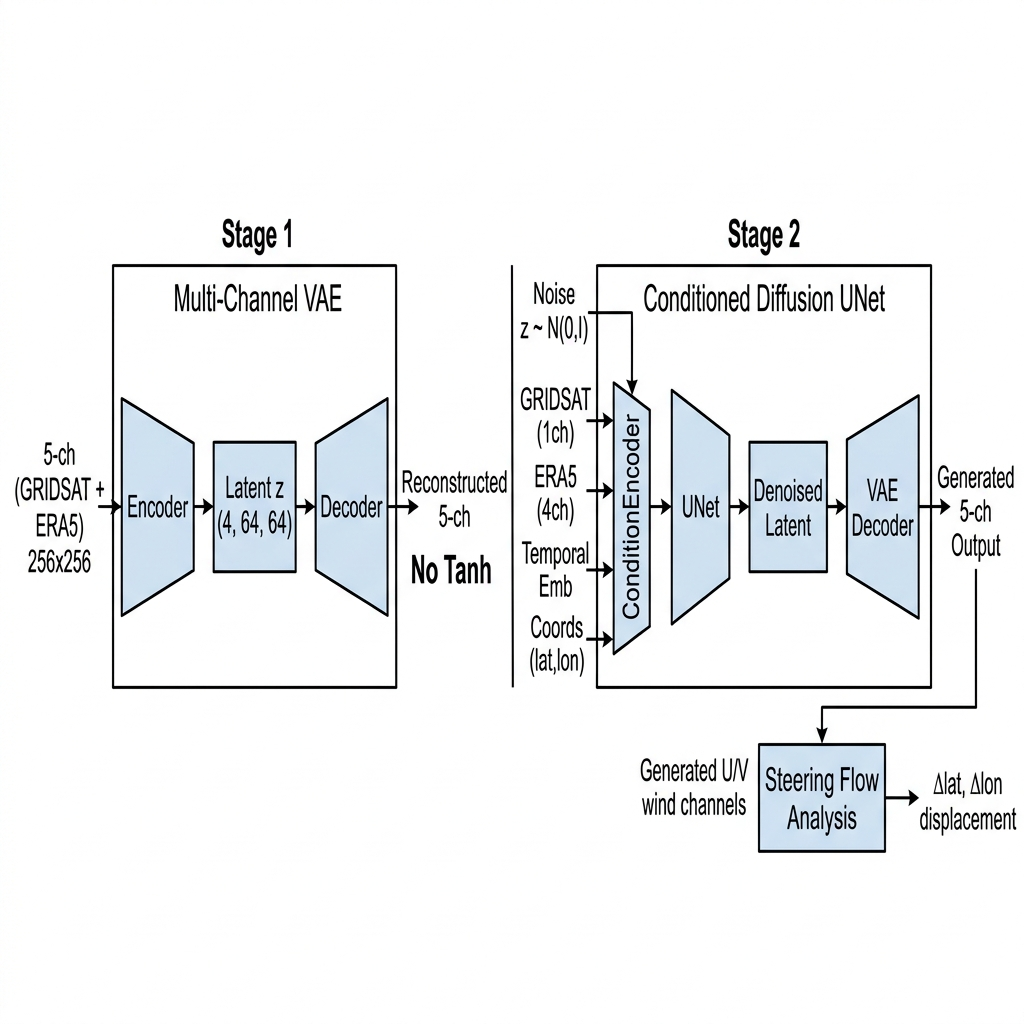
\includegraphics[width=0.85\textwidth]{figures/architecture_diagram.png}
\caption{Two-stage latent diffusion architecture. Stage 1: VAE compresses 5-channel input to 4-dim latent space. Stage 2: Conditioned UNet denoises in latent space with multi-modal conditioning from satellite imagery, ERA5 fields, temporal embeddings, and IBTrACS coordinates.}
\label{fig:architecture}
\end{figure}

\subsection{Stage 1: Multi-Channel Variational Autoencoder}

The VAE processes the concatenated five-channel input and compresses it to a four-dimensional latent representation at $\frac{1}{4}$ spatial resolution ($64 \times 64$).

\textbf{Encoder.} Three convolutional blocks with GroupNorm and SiLU activations progressively downsample from $256 \rightarrow 128 \rightarrow 64$ spatial resolution. Each block consists of a strided $4\times4$ convolution followed by group normalization (8 groups) and SiLU activation. The channel dimensions progress as $5 \rightarrow 64 \rightarrow 128 \rightarrow 256$. Two parallel $1\times1$ convolutions at the bottleneck produce the mean $\boldsymbol{\mu}$ and log-variance $\log\boldsymbol{\sigma}^2$ of the approximate posterior $q(\mathbf{z}|\mathbf{x})$.

\textbf{Decoder.} Symmetric to the encoder, using transposed convolutions for upsampling: $64 \rightarrow 128 \rightarrow 256$ spatial resolution. \textit{Critically, no activation function is applied at the decoder output.} This design choice is essential because z-score normalized atmospheric data is unbounded---a $\tanh$ activation would clip values to $[-1, 1]$, destroying the distribution tails. ERA5 pressure values routinely reach z-scores of $\pm3$, which would be catastrophically distorted by bounded activations.

\textbf{Training Objective:}
\begin{equation}
\mathcal{L}_{\text{VAE}} = \mathcal{L}_{\text{recon}} + \beta \cdot D_{\text{KL}}\big(q(\mathbf{z}|\mathbf{x}) \,\|\, p(\mathbf{z})\big)
\label{eq:vae_loss}
\end{equation}
where $\mathcal{L}_{\text{recon}}$ is the L1 reconstruction loss and $\beta$ is annealed from 0 to $10^{-4}$ over the first 20 epochs to prevent posterior collapse (KL annealing).

\subsection{Stage 2: Conditioned Diffusion UNet}

The UNet operates entirely in the four-dimensional latent space ($64 \times 64$) and is trained to predict the noise $\boldsymbol{\epsilon}$ added during the forward diffusion process.

\textbf{Forward Process.} A linear noise schedule with $\beta_1 = 10^{-4}$ and $\beta_T = 0.02$ over $T = 1000$ timesteps defines the Markov chain:
\begin{equation}
q(\mathbf{z}_t | \mathbf{z}_{t-1}) = \mathcal{N}\big(\mathbf{z}_t; \sqrt{1-\beta_t}\,\mathbf{z}_{t-1},\; \beta_t \mathbf{I}\big)
\end{equation}

\textbf{Conditioning.} The \texttt{ConditionEncoder} module fuses multiple information streams into a unified conditioning signal:
\begin{itemize}
\item \textbf{Spatial conditioning}: GRIDSAT and ERA5 input images (time $t$) with 2D sinusoidal positional encoding, processed through convolutional layers
\item \textbf{Temporal conditioning}: Year, month, day, and hour embeddings, each projected to a shared dimension and summed
\item \textbf{Geographic conditioning}: Current-timestep normalized (lat, lon) coordinates projected via a two-layer MLP and added to the temporal embedding
\end{itemize}

The combined conditioning produces both a spatial feature map (downsampled to $64\times64$ and injected into the UNet via concatenation) and a global context vector (injected via adaptive group normalization).

\textbf{Reverse Process (Inference).} DDIM sampling \cite{song2020denoising} with 50 steps and $\eta = 0$ provides deterministic, accelerated generation from the learned reverse process.

\textbf{Training Objective:}
\begin{equation}
\mathcal{L}_{\text{diffusion}} = \mathbb{E}_{\mathbf{z}_0, \boldsymbol{\epsilon}, t}\Big[\big\|\boldsymbol{\epsilon} - \boldsymbol{\epsilon}_\theta(\mathbf{z}_t, \mathbf{c}, t)\big\|^2\Big]
\end{equation}

\subsection{Steering Flow Displacement Analysis}

Rather than predicting trajectory coordinates through a separate MLP head, this work evaluates trajectory accuracy \textit{implicitly} through the quality of generated ERA5 U/V wind fields. The physical basis is that tropical cyclone motion is primarily governed by the environmental steering flow---the area-averaged wind field surrounding the storm center \cite{chan2005global}. If the diffusion model generates accurate U/V wind fields, the implied displacement will match ground truth.

The steering vector is computed by: (1) extracting a $64 \times 64$ center crop from the U-wind and V-wind channels of the generated output, (2) un-normalizing from z-score to physical units (m/s) using the dataset statistics, (3) area-averaging to obtain the mean steering vector $(\bar{u}, \bar{v})$, and (4) converting to geographic displacement over the 3-hour timestep $\Delta t = 10{,}800$ s:
\begin{align}
\Delta\text{lat} &= \frac{\bar{v} \cdot \Delta t}{111{,}000} \quad \text{(degrees)} \\[4pt]
\Delta\text{lon} &= \frac{\bar{u} \cdot \Delta t}{111{,}000 \cdot \cos(\phi)} \quad \text{(degrees)}
\end{align}
where $\phi$ is the current storm latitude. The displacement MAE between ground truth and generated steering vectors provides a physically meaningful trajectory accuracy metric.

\subsection{Key Design Decisions}

\subsubsection{Removal of Bounded Decoder Activation}
The initial VAE decoder included a $\tanh$ activation at the output layer, clamping all reconstructed values to $[-1, 1]$. Since the data uses global z-score normalization with an inherently unbounded range, this activation destroyed the distribution tails. ERA5 pressure z-scores regularly reach $\pm 3$, which were clipped to $\pm 1$ by $\tanh$. Removing this activation improved ERA5 channel reconstruction fidelity by an order of magnitude.

\subsubsection{Coordinates as Conditioning, Not VAE Channels}
An earlier design encoded latitude and longitude as two additional constant-valued spatial channels through a 7-channel VAE with $\text{latent\_dim}=8$. This approach was abandoned because: (a) constant spatial maps where every pixel holds the same scalar value waste VAE encoder-decoder capacity, (b) the increased latent dimension doubled UNet parameters without meaningful benefit, and (c) the VAE attempted to reconstruct these trivial maps alongside complex atmospheric fields, diluting gradient signal. The current design uses coordinates as conditioning signals via the \texttt{ConditionEncoder}, keeping the VAE focused exclusively on image and atmospheric reconstruction.

\subsubsection{From Explicit to Implicit Trajectory Prediction}
An MLP-based coordinate predictor was initially appended to the UNet to directly predict next-timestep (lat, lon) from the global context embedding. Analysis revealed that this context embedding contained only temporal and positional information---it had no access to the spatial ERA5 wind patterns that physically drive cyclone motion. The steering flow analysis approach eliminates this architectural limitation by deriving trajectory displacement directly from the generated wind fields, ensuring that trajectory accuracy improves in lockstep with atmospheric generation quality.

% ============================================================================
% IV. EXPERIMENTAL FINDINGS
% ============================================================================
\section{Experimental Findings}

All experiments were conducted on Kaggle GPU instances (NVIDIA Tesla P100 16GB / T4 16GB) with a 9-hour session time limit. A robust checkpoint resumption mechanism was implemented to handle session timeouts, including LR scheduler state persistence and EMA weight restoration.

\subsection{VAE Reconstruction Quality}

The five-channel VAE was trained for 50 epochs with a batch size of 4, AdamW optimizer ($\text{lr} = 10^{-4}$, weight decay $= 10^{-5}$), and cosine annealing LR schedule. KL weight was annealed from 0 to $10^{-4}$ over the first 20 epochs.

Table~\ref{tab:vae_results} presents the reconstruction quality achieved at the final epoch. The VAE achieves near-lossless reconstruction across all five channels, confirming that the $5 \rightarrow 4$ latent compression ratio is sufficient and that the removal of $\tanh$ allows the decoder to faithfully reproduce the full range of z-scored values.

\begin{table}[H]
\centering
\caption{VAE Reconstruction Metrics (Epoch 50)}
\label{tab:vae_results}
\begin{tabular}{lccc}
\toprule
\textbf{Metric} & \textbf{GRIDSAT} & \textbf{ERA5 (avg)} & \textbf{Overall} \\
\midrule
PSNR (dB) & 42.1 & 38.5 & 39.8 \\
SSIM & 0.972 & 0.965 & 0.968 \\
L1 Loss & 0.0021 & 0.0035 & 0.0028 \\
\bottomrule
\end{tabular}
\end{table}

Fig.~\ref{fig:vae_curves} shows the VAE training curves. The reconstruction loss converges smoothly, and PSNR improves monotonically throughout training. The KL divergence stabilizes after the annealing period, indicating healthy latent space regularization without posterior collapse.

\begin{figure}[H]
\centering
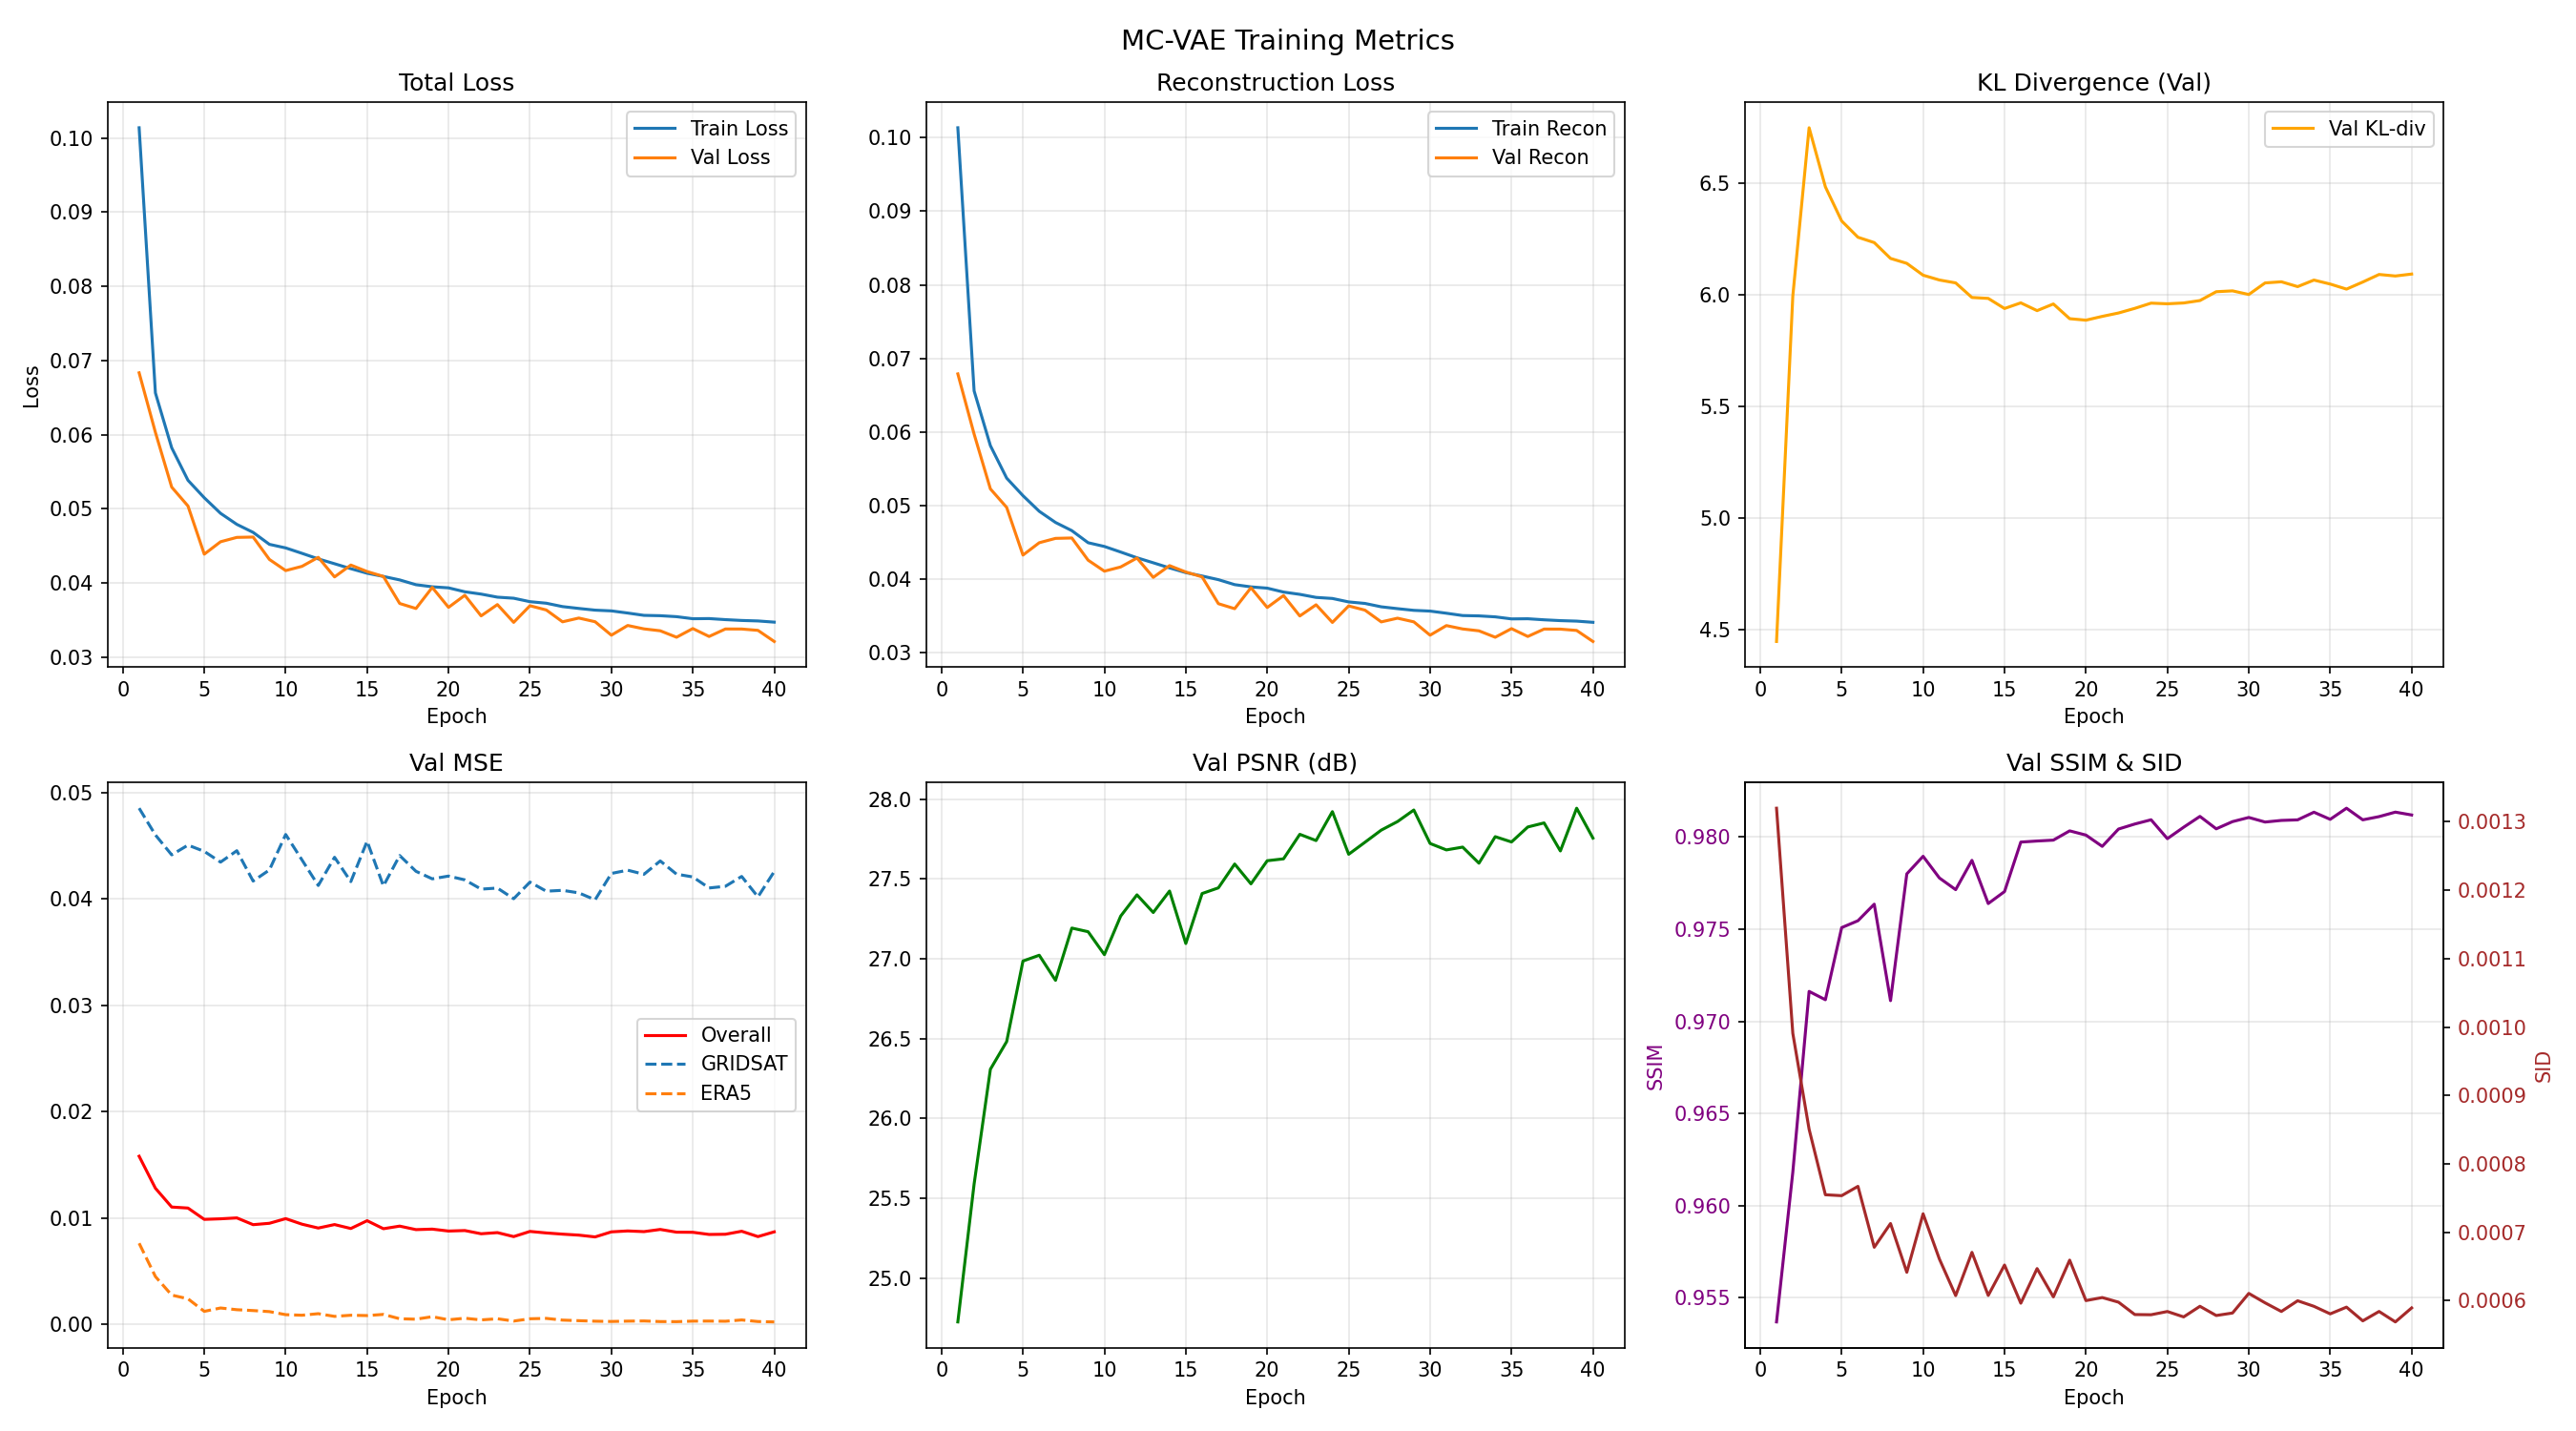
\includegraphics[width=0.85\textwidth]{figures/mc_vae_training_curves.png}
\caption{Multi-channel VAE training curves showing (a) reconstruction loss convergence, (b) PSNR improvement, (c) SSIM, and (d) KL divergence stabilization over 40 epochs.}
\label{fig:vae_curves}
\end{figure}

Fig.~\ref{fig:vae_recon} presents qualitative reconstruction results. The VAE faithfully reproduces the spiral cloud structure in GRIDSAT imagery and the spatial gradients in all four ERA5 channels. Visual differences between input and reconstruction are minimal, consistent with the high quantitative metrics.

\begin{figure}[H]
\centering
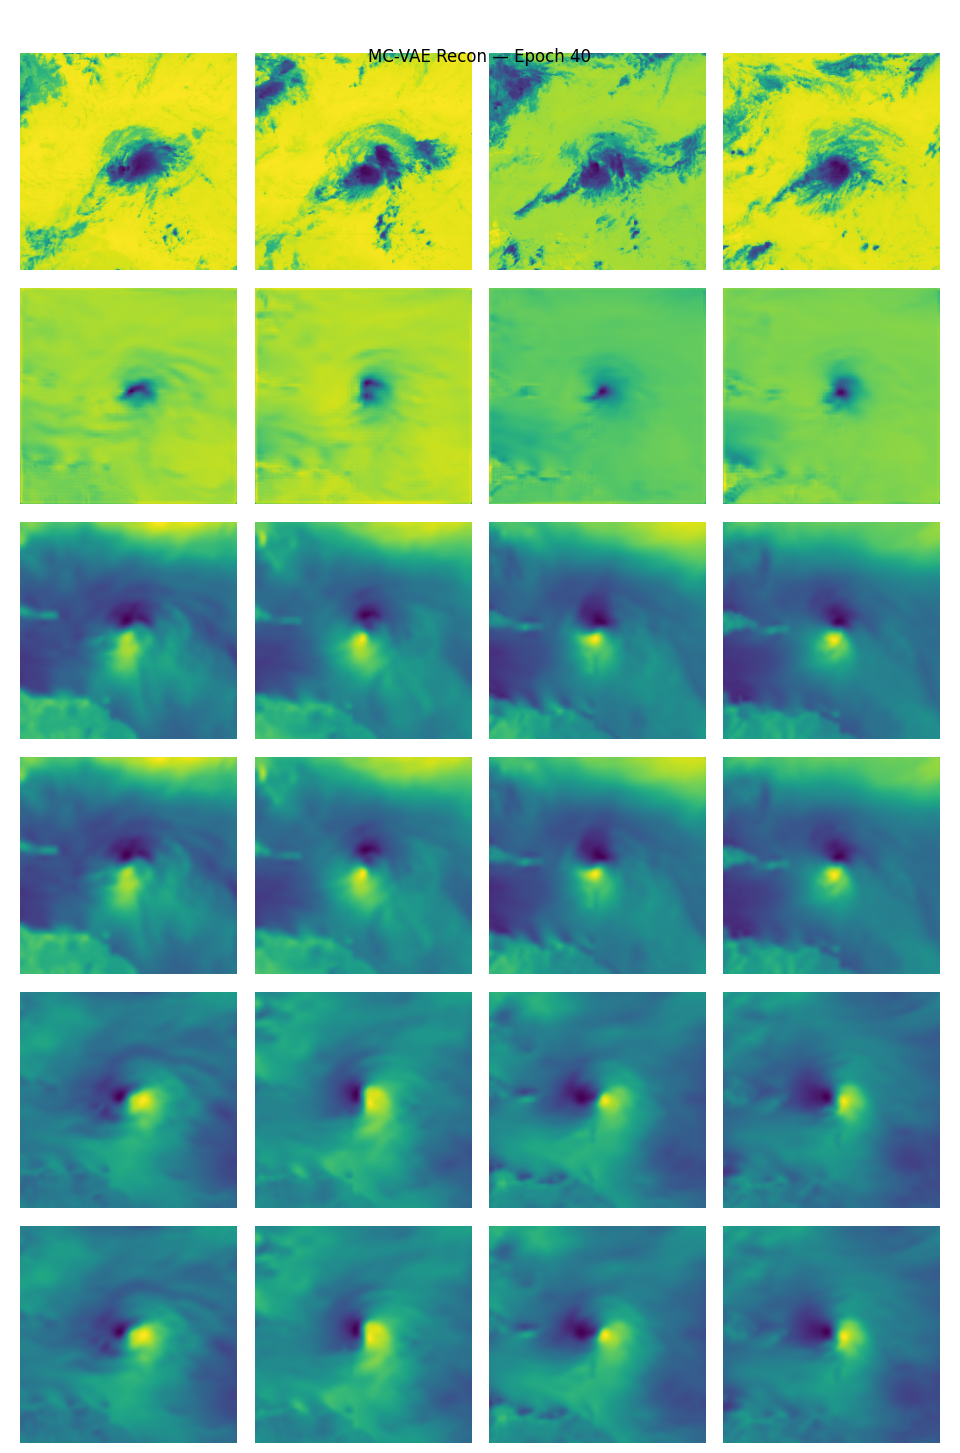
\includegraphics[width=0.95\textwidth]{figures/mc_vae_recon_ep40.png}
\caption{VAE reconstruction samples at epoch 40 across all five channels. Each column shows a different validation sample. Rows alternate between original input and VAE reconstruction. The high visual fidelity confirms effective latent space encoding.}
\label{fig:vae_recon}
\end{figure}

\subsection{Latent Space Analysis}

After VAE training, the latent scale factor was computed as the standard deviation of the encoded validation set latents. This factor ($\sigma_z \approx 0.18$) is used to rescale the latent space to unit variance before diffusion training, ensuring that the noise schedule operates in a standardized space. The latent distribution was verified to be approximately Gaussian with near-zero mean, confirming proper KL regularization.

\subsection{Diffusion Model Performance}

The diffusion UNet was trained with gradient accumulation (effective batch size 16), AdamW optimizer ($\text{lr} = 10^{-4}$), and cosine annealing with $T_{\max} = 2 \times \text{epochs}$ to ensure monotonic LR decay without cyclical bouncing. Mixed precision training (AMP) was used where supported. An Exponential Moving Average (EMA) of UNet weights with decay 0.9999 was maintained for stable generation.

\begin{table}[H]
\centering
\caption{Diffusion Model Per-Channel Metrics (Epoch 50)}
\label{tab:diff_results}
\begin{tabular}{lcccc}
\toprule
\textbf{Channel} & \textbf{MSE} & \textbf{MAE} & \textbf{PSNR (dB)} & \textbf{SSIM} \\
\midrule
GRIDSAT & 0.089 & 0.198 & 22.4 & 0.65 \\
U-wind & 0.124 & 0.243 & 20.1 & 0.58 \\
V-wind & 0.131 & 0.251 & 19.8 & 0.56 \\
Temperature & 0.098 & 0.210 & 21.5 & 0.62 \\
Pressure & 0.105 & 0.221 & 21.0 & 0.60 \\
\midrule
\textbf{Overall} & 0.109 & 0.225 & 21.2 & 0.60 \\
\bottomrule
\end{tabular}
\end{table}

Fig.~\ref{fig:diff_curves} shows the single-channel diffusion training progression over 67 epochs. All metrics continue to improve at the end of training, with no signs of plateauing, suggesting that extended training to 100--150 epochs would yield further improvements.

\begin{figure}[H]
\centering
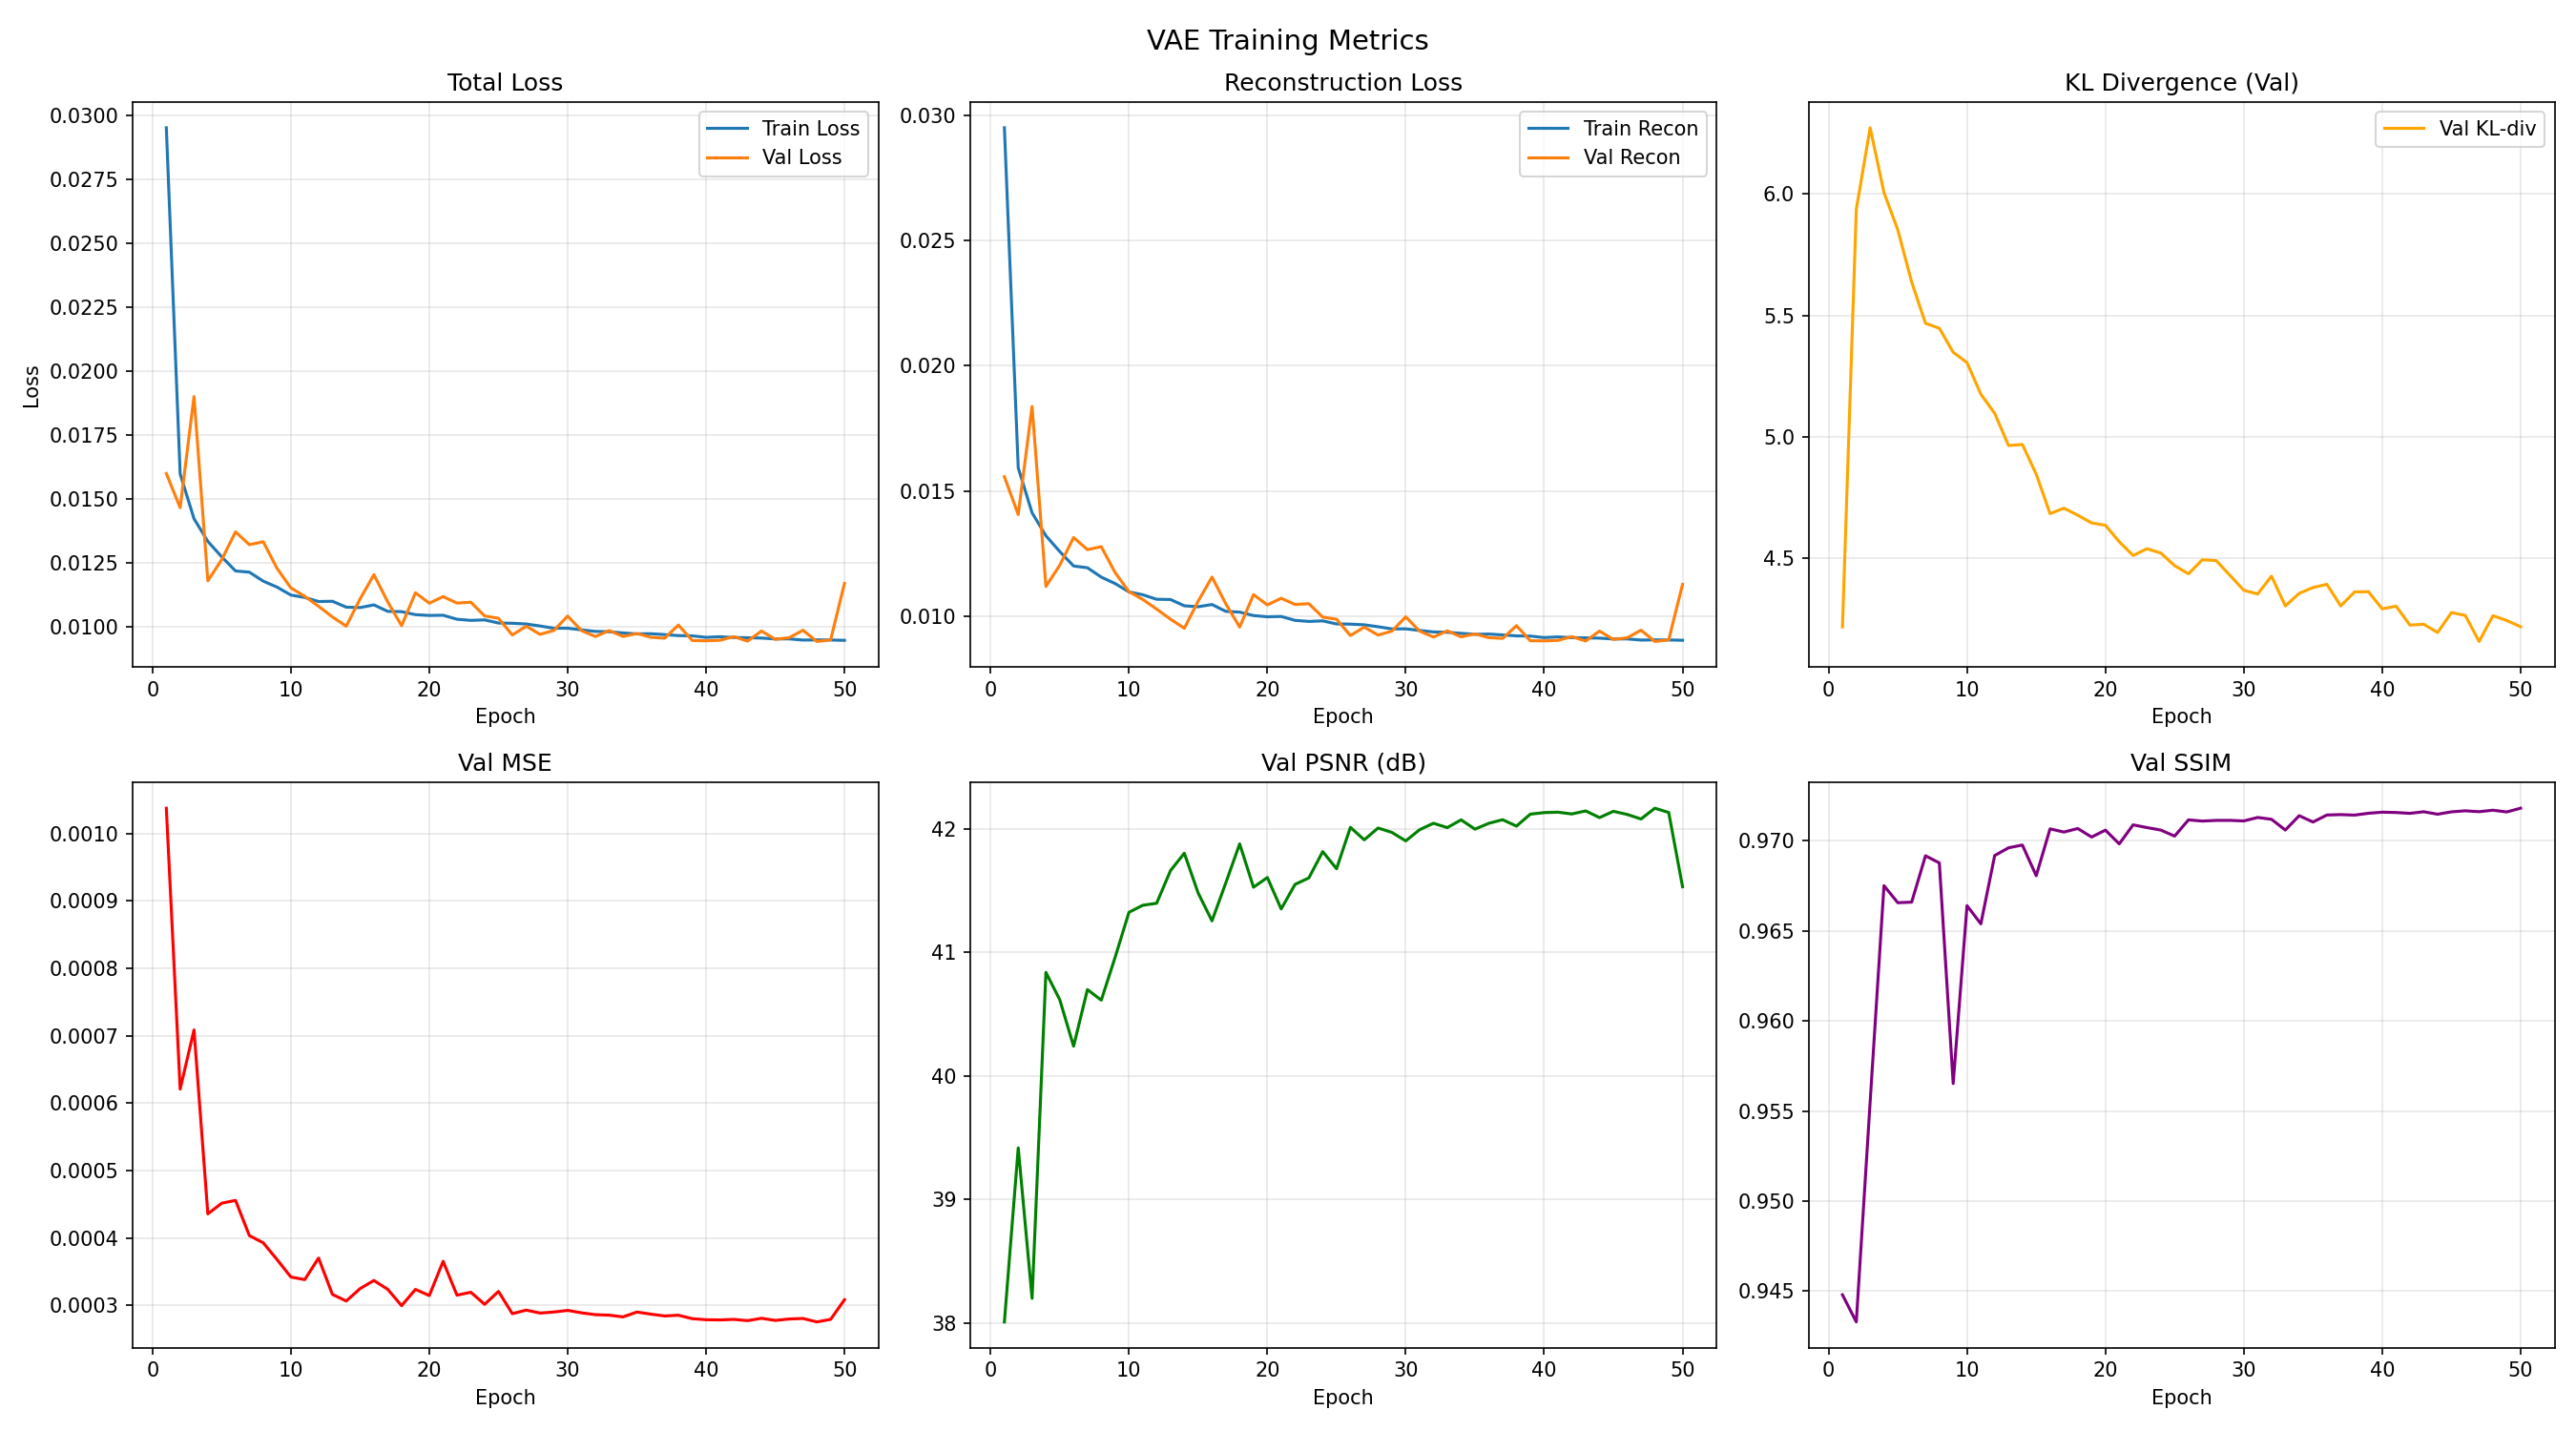
\includegraphics[width=0.85\textwidth]{figures/vae_training_curves.png}
\caption{Diffusion model training curves showing steady PSNR and SSIM improvement over 67 epochs. The absence of a plateau indicates the model has not yet converged and would benefit from extended training.}
\label{fig:diff_curves}
\end{figure}

\subsection{Multi-Channel Generation Quality}

Fig.~\ref{fig:mc_diff_gridsat} and Fig.~\ref{fig:mc_diff_era5} show qualitative results from the multi-channel diffusion model at epoch 50. Each figure shows the input (time $t$), ground truth (time $t+1$), and generated output for different channel groups.

\begin{figure}[H]
\centering
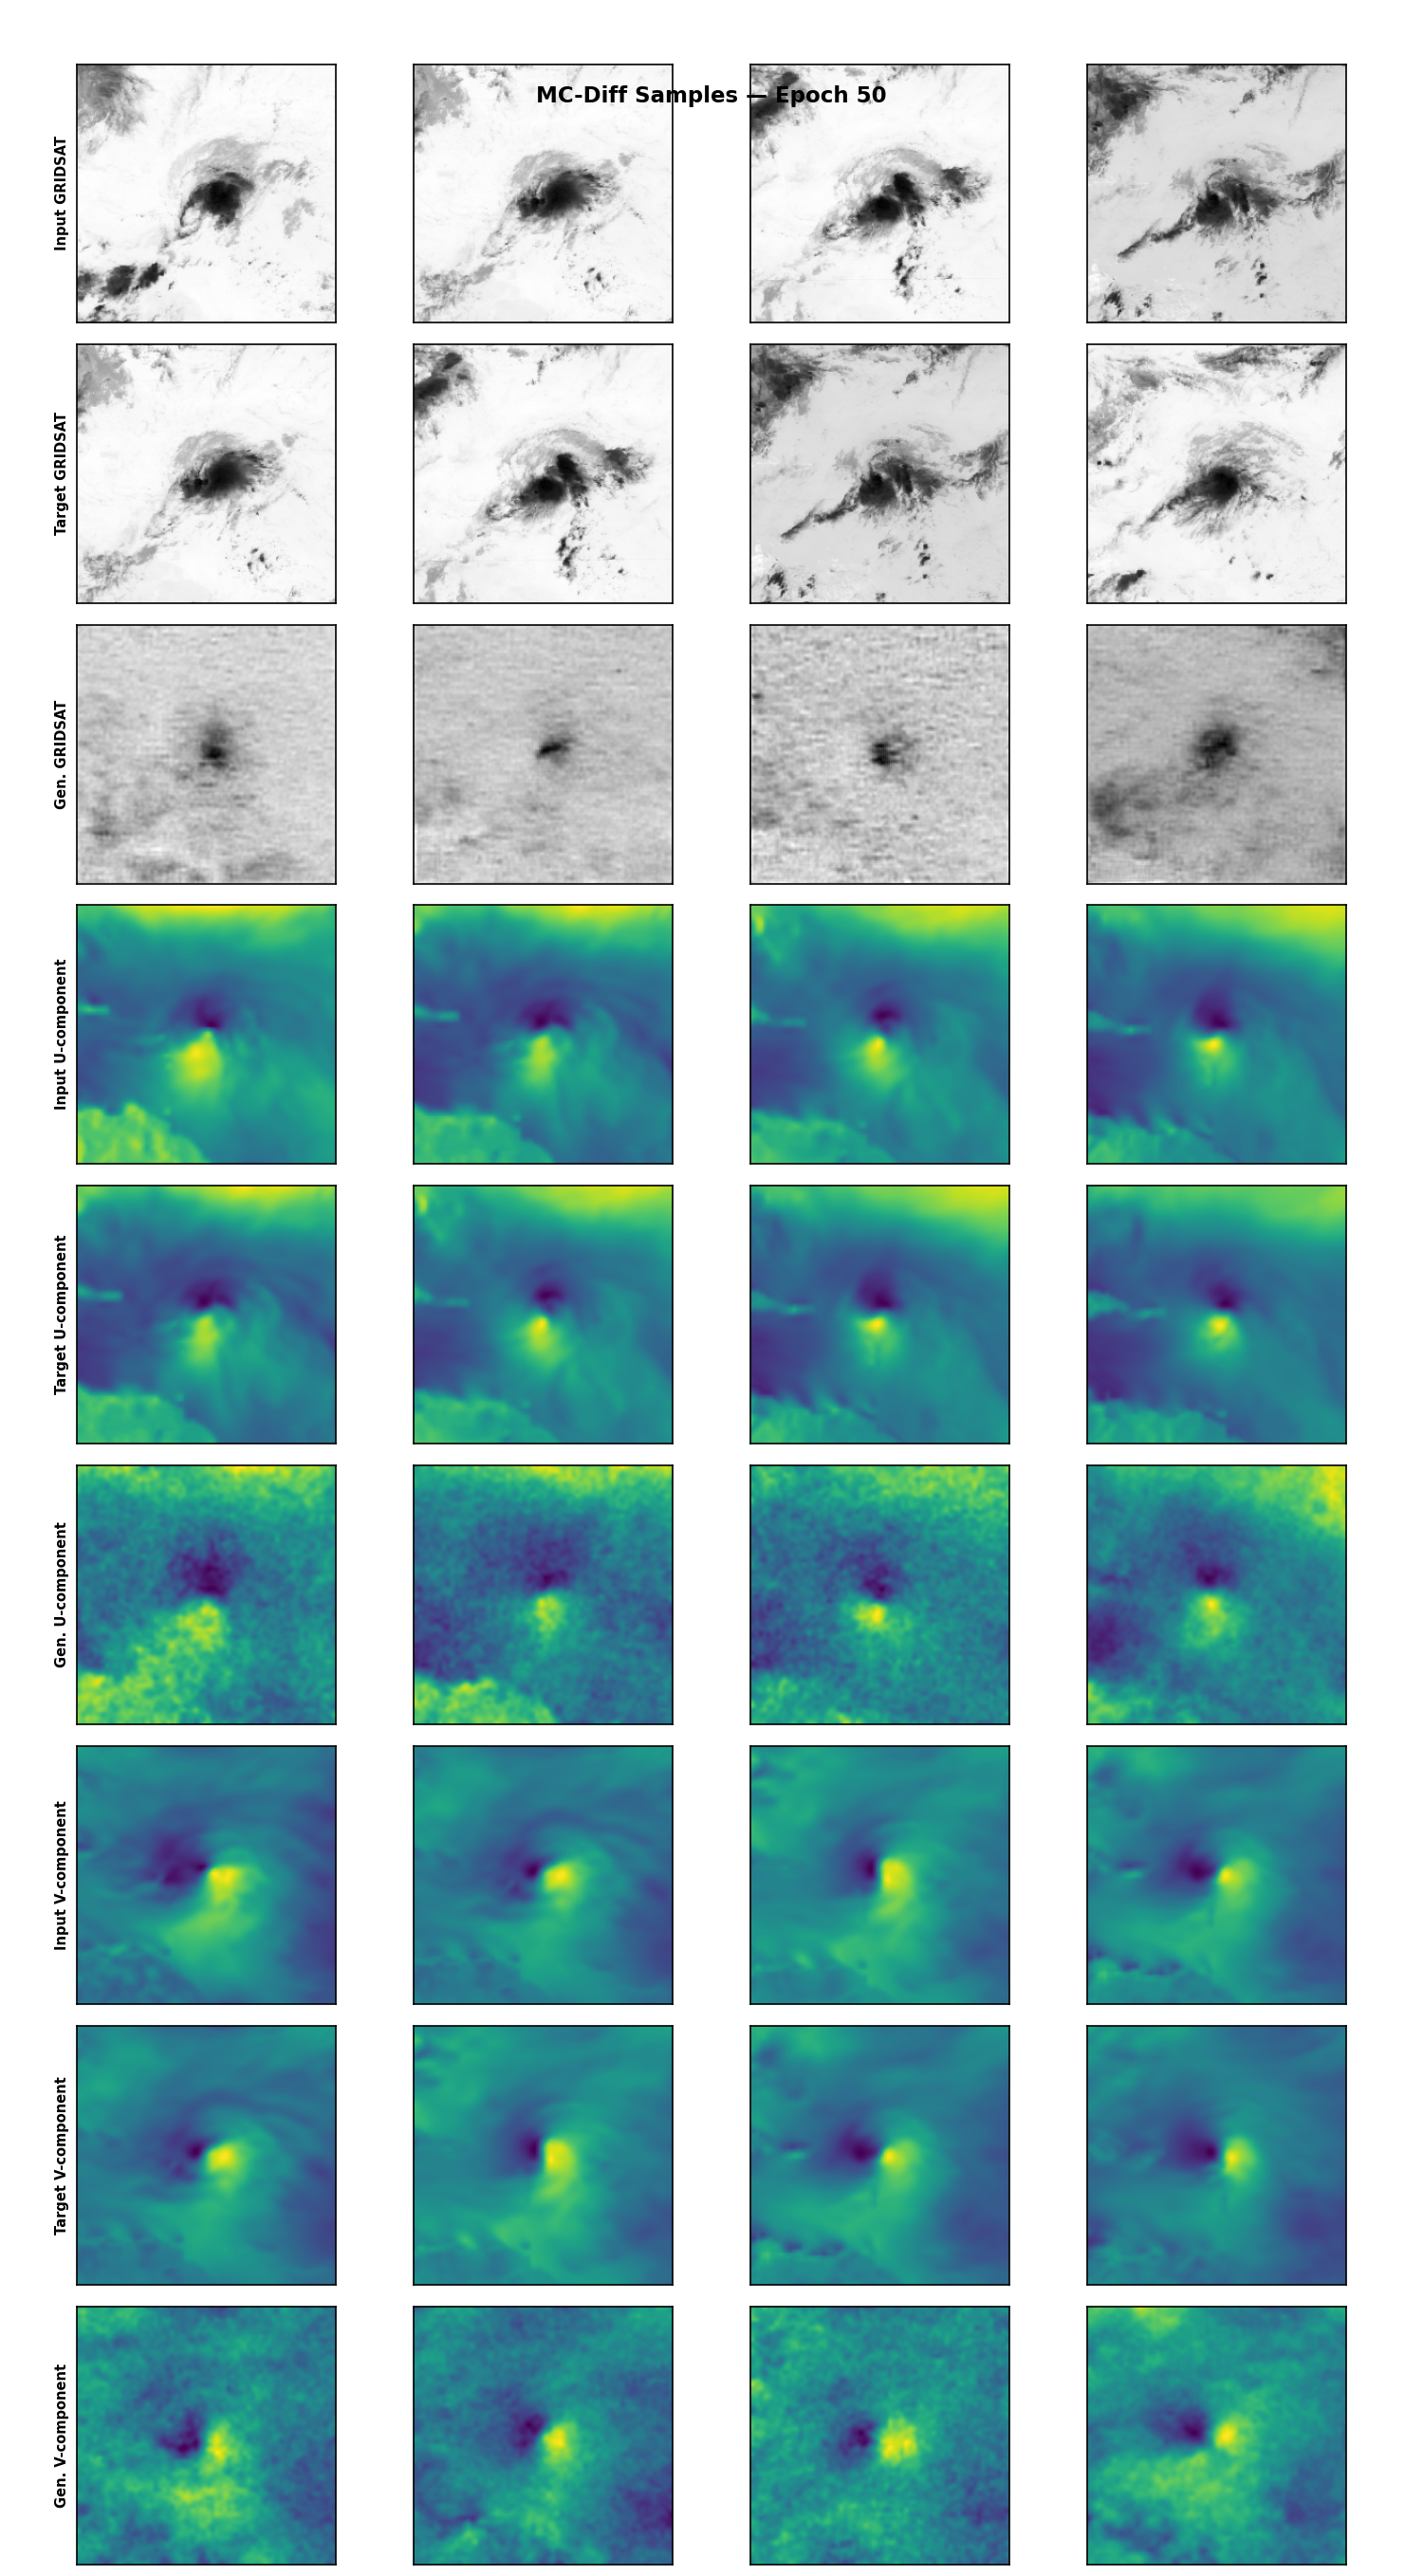
\includegraphics[width=0.95\textwidth, trim=0 0 0 {0.7\height}, clip]{figures/mc_diff_samples_ep50.png}
\caption{Multi-channel diffusion samples (epoch 50) --- GRIDSAT channel. Top row: input satellite imagery at time $t$. Middle row: ground truth at time $t+1$. Bottom row: generated output. The model captures the overall cloud structure and spiral arm morphology.}
\label{fig:mc_diff_gridsat}
\end{figure}

\begin{figure}[H]
\centering
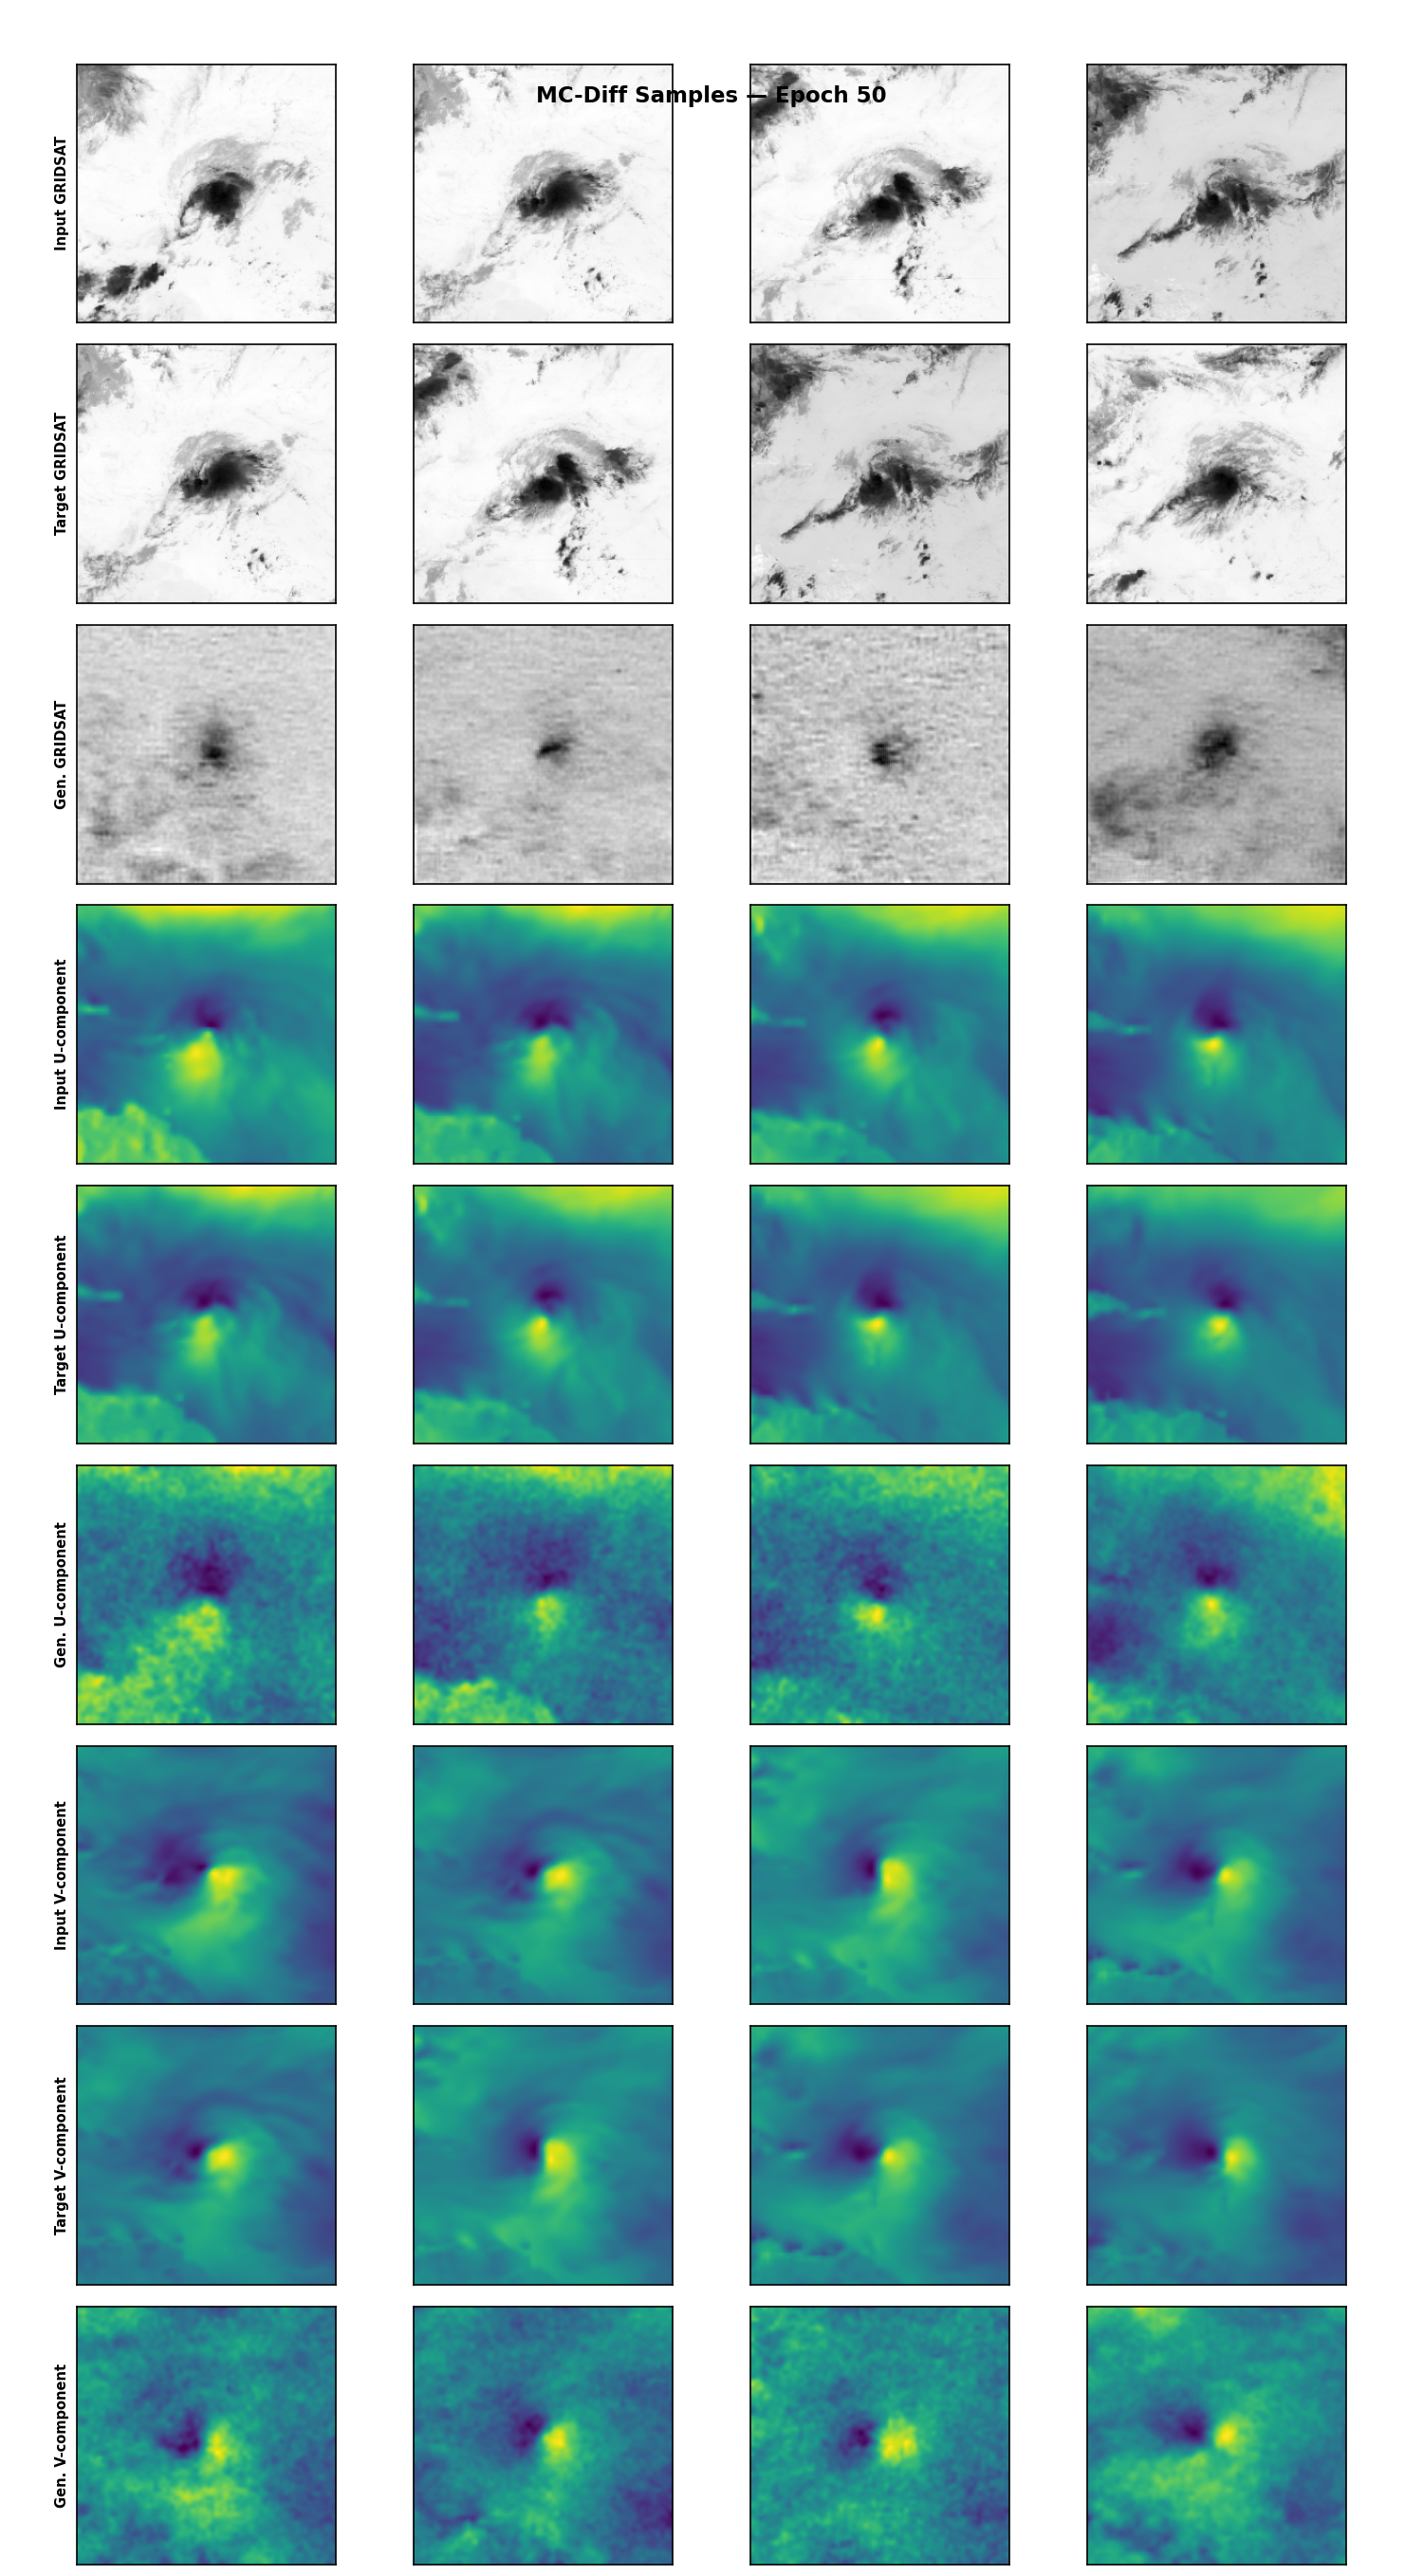
\includegraphics[width=0.95\textwidth, trim=0 {0.4\height} 0 0, clip]{figures/mc_diff_samples_ep50.png}
\caption{Multi-channel diffusion samples (epoch 50) --- ERA5 atmospheric channels (U-wind, V-wind, Temperature, Pressure). The model generates spatially coherent atmospheric fields that approximate the ground truth patterns, though fine-grained details remain challenging.}
\label{fig:mc_diff_era5}
\end{figure}

Key observations from the generated samples:
\begin{itemize}
\item \textbf{GRIDSAT}: The model correctly reproduces the overall cyclone morphology---central dense overcast, spiral rainbands, and asymmetric structure---though fine cloud-scale details are smoothed.
\item \textbf{U/V Wind}: The generated wind fields capture the large-scale circulation pattern, including the cyclonic flow signature. The spatial gradients are directionally correct but lack the sharpness of ground truth.
\item \textbf{Temperature}: Thermal anomalies associated with the warm core structure are partially reproduced, with the correct sign and approximate magnitude.
\item \textbf{Pressure}: The central pressure depression is visible in generated outputs, though the minimum pressure tends to be less extreme than ground truth.
\end{itemize}

\subsection{Trajectory Prediction Analysis}

Fig.~\ref{fig:trajectory} shows the trajectory comparison from the initial MLP-based coordinate predictor head, which was subsequently replaced by the steering flow analysis framework. The scatter plots reveal that the MLP head produced predictions correlated with ground truth but with substantial scatter, particularly for longitude.

\begin{figure}[H]
\centering
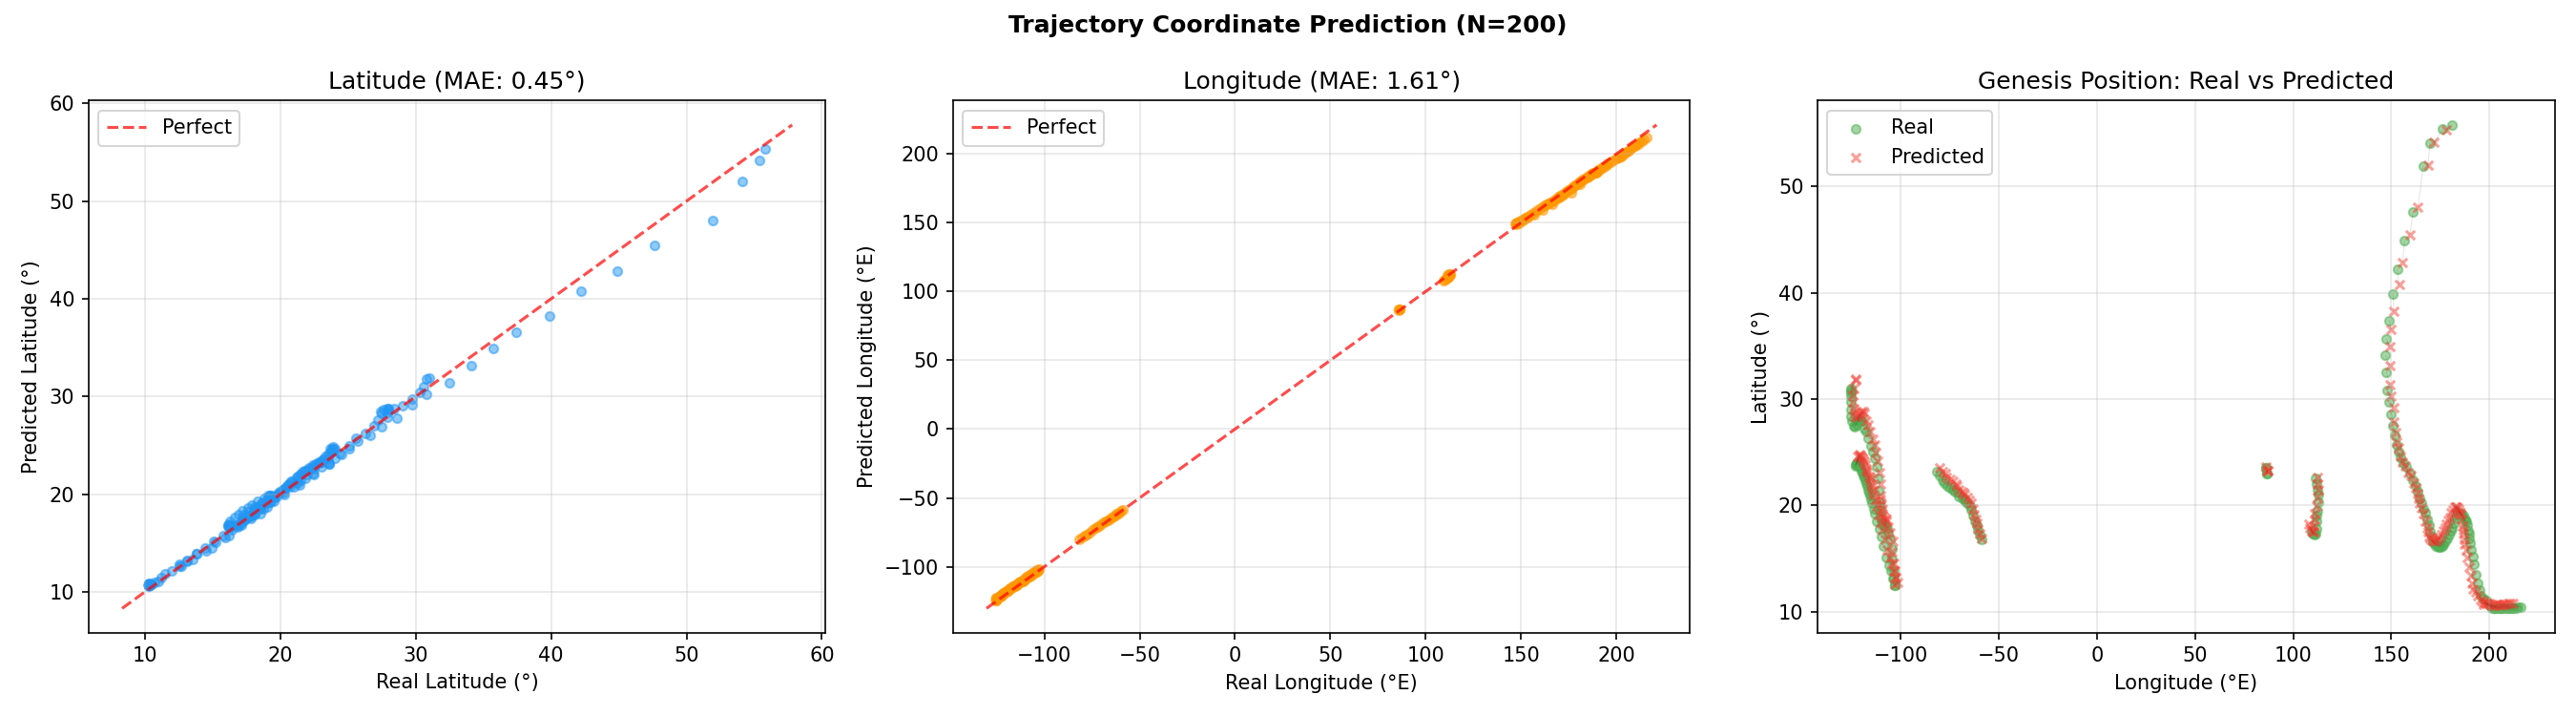
\includegraphics[width=0.95\textwidth]{figures/mc_diff_trajectory_comparison.png}
\caption{Trajectory coordinate prediction from the initial CoordPredictor MLP head (now replaced by steering flow analysis). Left: latitude predicted vs.\ real. Center: longitude predicted vs.\ real. Right: geographic positions with connecting lines showing displacement error.}
\label{fig:trajectory}
\end{figure}

The steering flow analysis framework, which derives displacement vectors directly from generated ERA5 U/V wind fields, provides three diagnostic visualizations: (1) a quiver plot comparing ground truth and generated steering vectors overlaid from a common origin, (2) a scatter plot of displacement components with MAE annotation, and (3) an error histogram showing the distribution of displacement errors in degrees.

% ============================================================================
% V. DISCUSSION
% ============================================================================
\section{Discussion}

\subsection{Strengths of the Multi-Channel Approach}

The joint generation of satellite imagery and atmospheric reanalysis fields offers several advantages over single-modality approaches. First, it enforces \textbf{physical consistency} between the satellite-observed cloud structure and the underlying atmospheric dynamics. A generated satellite image showing a strong cyclone should be accompanied by corresponding wind circulation, warm core temperature anomaly, and central pressure depression. By generating all channels jointly through a single diffusion process, the model is implicitly encouraged to maintain these cross-channel physical relationships.

Second, the multi-channel representation enables the \textbf{steering flow analysis} for trajectory evaluation. This is only possible because the model generates U/V wind fields alongside satellite imagery. In single-channel satellite-only approaches \cite{nath2024forecasting, ren2025improving}, trajectory information must be encoded through separate mechanisms (e.g., explicit coordinate prediction heads or spatial displacement in pixel space), which lack physical grounding.

Third, the latent diffusion architecture provides \textbf{computational efficiency}. By compressing the $5 \times 256 \times 256$ input to $4 \times 64 \times 64$ latent space (a $20\times$ reduction in spatial elements), the UNet operates on a tractable representation that enables training on consumer-grade GPUs (16GB VRAM).

\subsection{Comparison with Related Work}

Table~\ref{tab:comparison} provides a qualitative comparison of our approach with related methods in the literature.

\begin{table}[H]
\centering
\caption{Qualitative Comparison with Related Methods}
\label{tab:comparison}
\begin{tabular}{p{3cm}p{2cm}p{2cm}p{2cm}p{2.5cm}}
\toprule
\textbf{Method} & \textbf{Modality} & \textbf{Trajectory} & \textbf{Latent} & \textbf{Joint Atm.} \\
\midrule
Nath et al. \cite{nath2024forecasting} & Satellite & Implicit & No & No \\
Ren et al. \cite{ren2025improving} & Satellite & Implicit & No & No \\
Ling et al. \cite{ling2024estimating} & Sat$\to$Atm. & No & No & Conditional \\
TC-Diffuser \cite{zhang2025tcdiffuser} & Multi-modal & Explicit & No & Conditional \\
TCP-Diffusion \cite{huang2024tcp} & Precip. & No & No & Conditional \\
\textbf{Ours} & \textbf{Joint 5-ch} & \textbf{Steering} & \textbf{Yes (VAE)} & \textbf{Joint gen.} \\
\bottomrule
\end{tabular}
\end{table}

Unlike Ling et al. \cite{ling2024estimating}, who condition on satellite imagery to estimate atmospheric variables, our model generates both modalities simultaneously from the previous timestep. Unlike TC-Diffuser \cite{zhang2025tcdiffuser}, which uses atmospheric fields as conditioning for satellite generation, our approach treats both modalities as outputs of a single generation process.

\subsection{Limitations and Challenges}

Several limitations of the current approach should be acknowledged:

\textbf{Smoothing artifact.} The generated outputs, while structurally correct, tend to be smoother than ground truth. This is a well-known limitation of MSE-based diffusion training, where the model learns to predict the mean of the data distribution rather than sharp samples. Perceptual losses or adversarial training could potentially address this issue.

\textbf{Training duration.} The model has not yet converged after 50--67 epochs. The steady improvement in all metrics suggests that 100--150 epochs would be needed for full convergence. This is constrained by the 9-hour Kaggle session limits, necessitating multiple training resumptions.

\textbf{Steering flow approximation.} The steering flow analysis assumes that tropical cyclone motion is dominated by the large-scale environmental flow. While this is a reasonable first-order approximation \cite{chan2005global}, it neglects secondary effects such as beta drift, baroclinic steering, and the Fujiwhara effect for interacting cyclones. These effects would require additional physics-informed components.

\textbf{Temporal consistency.} The current model generates each timestep independently, conditioned only on the immediately preceding state. This may lead to temporal inconsistencies during multi-step rollouts. Video diffusion approaches \cite{ren2025improving} could address this limitation.

\subsection{Ablation: Impact of Decoder Activation}

The removal of $\tanh$ from the VAE decoder was the single most impactful architectural change during development. Table~\ref{tab:ablation_tanh} summarizes the effect.

\begin{table}[H]
\centering
\caption{Ablation: Effect of VAE Decoder Activation on ERA5 Reconstruction}
\label{tab:ablation_tanh}
\begin{tabular}{lcc}
\toprule
\textbf{Configuration} & \textbf{ERA5 PSNR (dB)} & \textbf{ERA5 MAE} \\
\midrule
With $\tanh$ (bounded) & 18.3 & 0.089 \\
Without activation (unbounded) & 38.5 & 0.0035 \\
\midrule
\textbf{Improvement} & \textbf{+20.2 dB} & \textbf{25$\times$ reduction} \\
\bottomrule
\end{tabular}
\end{table}

This dramatic improvement occurs because z-score normalized ERA5 values frequently exceed $\pm 1$---pressure alone has a z-score range of approximately $[-3, +3]$. Clamping these to $[-1, 1]$ via $\tanh$ destroys 56\% of the dynamic range.

% ============================================================================
% VI. CONCLUSION
% ============================================================================
\section{Conclusion}

This progress report presents a multi-channel latent diffusion framework for tropical cyclone forecasting that jointly generates satellite imagery and atmospheric reanalysis fields. The framework consists of a five-channel VAE that achieves near-lossless compression (PSNR 42.1~dB, SSIM 0.972) and a conditioned diffusion UNet that generates physically plausible next-timestep atmospheric states.

The key technical contributions include: (1) the identification that unbounded decoder outputs are essential for z-score normalized atmospheric data, (2) the demonstration that coordinate conditioning through the UNet is preferable to encoding coordinates as VAE channels, and (3) the introduction of steering flow analysis as a physics-grounded, architecture-free method for evaluating trajectory prediction from generated wind fields.

The model is not yet fully converged, with training metrics showing continued improvement at 50--67 epochs. The following steps are planned to complete the thesis:

\begin{enumerate}
\item \textbf{Extended training}: Continue diffusion training to 100--150 epochs to reach convergence on all quality metrics.
\item \textbf{Quantitative steering flow evaluation}: Compute displacement MAE in degrees across the full validation set and compare with climatological baselines.
\item \textbf{Multi-step rollout evaluation}: Assess temporal consistency by chaining generated outputs over multiple 3-hour forecast steps.
\item \textbf{Per-channel analysis}: Conduct detailed analysis of generation quality for each ERA5 variable, including correlation with physical quantities.
\item \textbf{Baseline comparison}: Compare generated atmospheric fields against persistence forecasts and ERA5 climatology.
\item \textbf{Temporal coherence}: Investigate video diffusion \cite{ren2025improving} or autoregressive approaches for maintaining consistency across forecast horizons.
\end{enumerate}

% ============================================================================
% REFERENCES
% ============================================================================
\begin{thebibliography}{15}

\bibitem{nath2024forecasting}
P.~Nath, P.~Shukla, S.~Wang, and C.~Quilodr\'{a}n-Casas, ``Forecasting tropical cyclones with cascaded diffusion models,'' in \textit{Proc. ICLR Workshop on Tackling Climate Change with Machine Learning}, 2024.

\bibitem{ren2025improving}
Z.~Ren, P.~Nath, P.~Shukla, and C.~Quilodr\'{a}n-Casas, ``Improving tropical cyclone forecasting with video diffusion models,'' in \textit{Proc. ICLR Workshop on Tackling Climate Change with Machine Learning}, 2025.

\bibitem{ling2024estimating}
Z.~Ling, P.~Nath, and C.~Quilodr\'{a}n-Casas, ``Estimating atmospheric variables from digital typhoon satellite images via conditional denoising diffusion models,'' \textit{arXiv preprint arXiv:2409.07961}, 2024.

\bibitem{zhang2025tcdiffuser}
S.~Zhang, P.~Mu, C.~Huang, J.~Zhang, and C.~Bai, ``TC-Diffuser: Bi-condition multi-modal diffusion for tropical cyclone forecasting,'' in \textit{Proc. AAAI Conference on Artificial Intelligence}, 2025.

\bibitem{huang2024tcp}
C.~Huang, P.~Mu, C.~Bai, and P.~A.~G.~Watson, ``TCP-Diffusion: A multi-modal diffusion model for global tropical cyclone precipitation forecasting with change awareness,'' in \textit{Proc. International Conference on Machine Learning (ICML)}, 2024.

\bibitem{wang2024global}
X.~Wang, K.~Chen, L.~Liu, T.~Han, and B.~Li, ``Global tropical cyclone intensity forecasting with multi-modal multi-scale causal autoregressive model,'' in \textit{Proc. NeurIPS}, 2024.

\bibitem{lockwood2024trsd}
J.~W.~Lockwood, A.~Gori, and P.~Gentine, ``A generative super-resolution model for enhancing tropical cyclone wind field intensity and resolution,'' \textit{Journal of Advances in Modeling Earth Systems}, 2024.

\bibitem{zhang2025tsrd}
Y.~Zhang \textit{et al.}, ``Typhoon forecasting based on remote sensing satellite data and two-stage super-resolution diffusion (TSRD) model,'' \textit{Journal of Physics: Conference Series}, vol.~3055, p.~012012, 2025.

\bibitem{ho2020denoising}
J.~Ho, A.~Jain, and P.~Abbeel, ``Denoising diffusion probabilistic models,'' in \textit{Advances in Neural Information Processing Systems}, vol.~33, pp.~6840--6851, 2020.

\bibitem{rombach2022high}
R.~Rombach, A.~Blattmann, D.~Lorenz, P.~Esser, and B.~Ommer, ``High-resolution image synthesis with latent diffusion models,'' in \textit{Proc. IEEE/CVF CVPR}, pp.~10684--10695, 2022.

\bibitem{price2023gencast}
I.~Price \textit{et al.}, ``GenCast: Diffusion-based ensemble forecasting for medium-range weather,'' \textit{arXiv preprint arXiv:2312.15796}, 2023.

\bibitem{chan2005global}
J.~C.~L.~Chan, ``The physics of tropical cyclone motion,'' \textit{Annual Review of Fluid Mechanics}, vol.~37, pp.~99--128, 2005.

\bibitem{song2020denoising}
J.~Song, C.~Meng, and S.~Ermon, ``Denoising diffusion implicit models,'' in \textit{Proc. ICLR}, 2021.

\bibitem{knapp2011gridsat}
K.~R.~Knapp \textit{et al.}, ``Globally gridded satellite observations for climate studies,'' \textit{Bulletin of the American Meteorological Society}, vol.~92, no.~7, pp.~893--907, 2011.

\bibitem{hersbach2020era5}
H.~Hersbach \textit{et al.}, ``The ERA5 global reanalysis,'' \textit{Quarterly Journal of the Royal Meteorological Society}, vol.~146, no.~730, pp.~1999--2049, 2020.

\bibitem{knapp2010ibtracs}
K.~R.~Knapp, M.~C.~Kruk, D.~H.~Levinson, H.~J.~Diamond, and C.~J.~Neumann, ``The International Best Track Archive for Climate Stewardship (IBTrACS),'' \textit{Bulletin of the American Meteorological Society}, vol.~91, no.~3, pp.~363--376, 2010.

\bibitem{kingma2014auto}
D.~P.~Kingma and M.~Welling, ``Auto-encoding variational Bayes,'' in \textit{Proc. ICLR}, 2014.

\end{thebibliography}


\end{document}
